\chapter{ Predictive Display}
\label{ch_7:PDsply}
In the last chapter, it was shown using simulation that the time delay between the remote and local stations leads the system towards instability. In this chapter, first a predictive model controller for time delayed teleoperation is presented. Associated issues of time delay on human performance are then highlighted. To alleviate the problem of time delay in visual feedback, predictive display using a RGB-Depth sensor is  implemented.

\section {Time Delay Compensation}
Simulation of a time delayed system with pure pursuit model for human controller was presented in Chapter \ref{c6_simulation}.  Stability aspects with input delay to the human model was pointed out. In paper by Ollero \cite{ollero1995stability}, stability of pure pursuit with input delay is presented and for completeness it is briefly discussed in Appendix \ref{appendix_b}.   In view of the above theoretical analysis and the simulation results presented in Chapter \ref{c6_simulation}, it is required to design  a stabilizing controller to take care of large delays, e.g.,  0.8 sec. One such design based on model  predictive control is presented next.

 \begin{figure}
 	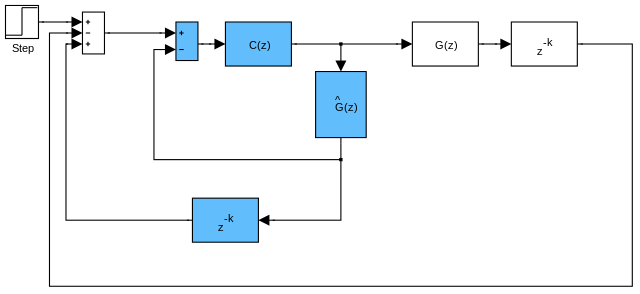
\includegraphics[width=\linewidth]{Chapter7/fig/Smith_predictor}
 	\caption{Smith predictor \cite{smith1959controller}}
 	\label{fig:Smith}
 \end{figure}
 
 One of the earliest predictor based controller for linear system with time delay  was proposed by Smith \cite{smith1959controller} called the Smith Predictor or Smith Controller. The schematic diagram of the smith controller is shown in Figure \ref{fig:Smith}. There are two loops, the inner and the outer loop, where $G(z)$ is the plant, $C(z)$ is the stabilizing controller  for the plant without delay, $\hat{G}(z)$ is the model of the plant.  As can be seen from  Figure \ref{fig:Smith}, during the period (k time unit ) when the feedback (output) is not available the model of the plant is used to predict the actual plant behaviour and generate the control signal accordingly. 
 
 In the presented case, the plant is the mobile robot developed in this PhD research. The block digram shown in Figure \ref{fig:blockdigTimeDelay} depicts the architecture of time delayed system which is applicable to the current mobile robot and the local station. The tele-operation  over wireless network for our system   resulted in a delay of $T_1= 500~ms$ with update frequency of 2Hz.  The delay was caused due to large amount of data being transmitted as  video feedback from the robot's onboard camera. Figure \ref{fig:delayphoto} shows the measured delay in the video link. The frequency of odometric and control  data exchange between the two stations was at the rate of 20Hz, i.e., a delay $T_2=50~ms$ only. This  loop runs  independent of the video feedback link.  It may be noted that $T_2<<T_1$.
 \begin{figure}[ht]
 	\centering
 	\begin{minipage}{0.55\textwidth}
 		\centering
 		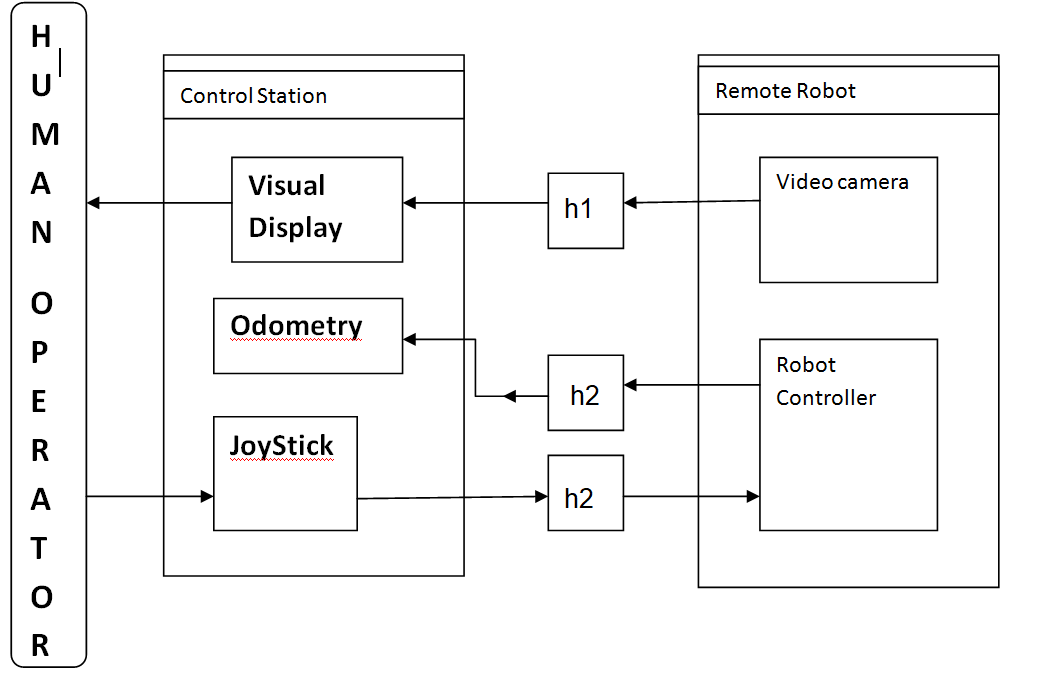
\includegraphics[width=.9\linewidth,keepaspectratio]{Chapter7/fig/BlockTimeDelay}
 		\captionof{figure}{Block digram of time \\delayed system}
 		\label{fig:blockdigTimeDelay}
 	\end{minipage}
  	\begin{minipage}{0.40\textwidth}
 	\centering
 	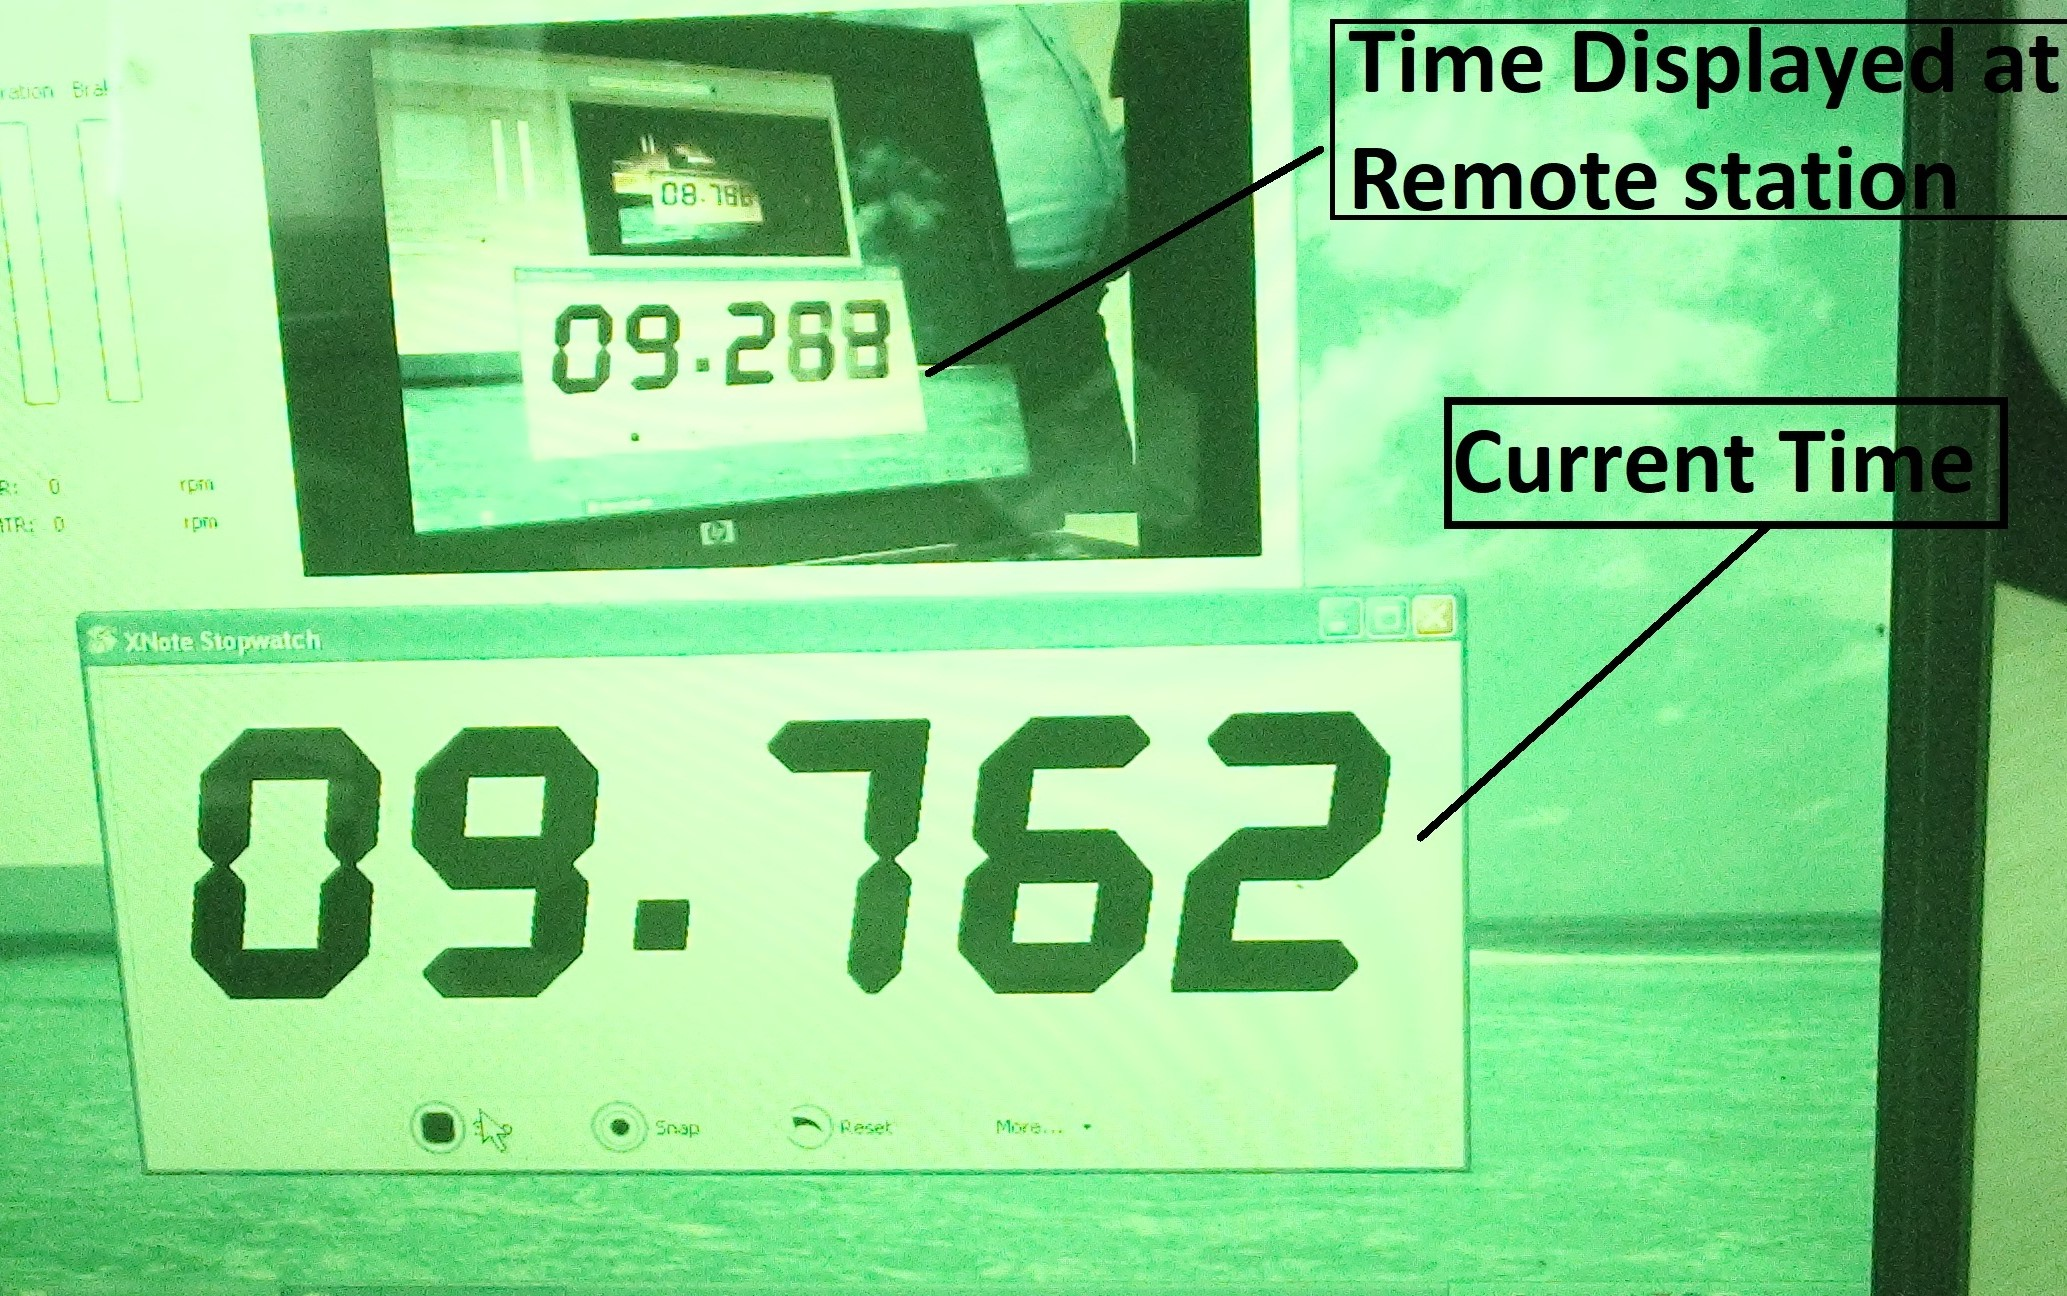
\includegraphics[width=\linewidth,keepaspectratio]{Chapter7/fig/delayMeasureNew}
 	\captionof{figure}{Delay measurment}
 	\label{fig:delayphoto}
 \end{minipage}%
 \end{figure} 


\subsection{Proposed controller}
The proposed control strategy to mitigate the effect of time delay is to predict the current position from the last known position, based on the delayed video image; using  the dynamic model of the mobile robot.  As shown in Figure \ref{fig:SmithRobot}, let us assume that we are at time $t+\delta$, but the latest pose  data of the robot available is that of at time $t$. The present pose at time $t+\delta$ was predicted  using  the dynamic model  of the robot derived in Chapter \ref{c4_Dynamics}, Equation \ref{CE}, and presented here again for convenience. 
\begin{equation}
\label{CE2}
\quad I(\theta)\ddot{\theta}=C(\theta,\dot{\theta})\dot{\theta}+\tau
\end{equation}
It may be noted that the dynamic model uses torque $\tau$ as its input, whereas the local station which uses pure pursuit for simulation of  human action   generates linear and angular velocities of the robot,  $v$ and $\omega$ as shown in Figure \ref{fig:SimBlock}. This is taken care by first converting $v \equiv\dot o_3$ and $\omega\equiv\omega_3$ to rear wheel velocities using Equations \ref{omegaPlat} and \ref{velPlat}. The rear wheel velocities  are then used in PI controller of the rear wheel motors to generate the $\tau$ for Equation \ref{CE2}.

This predicted position is given to the pure pursuit algorithm to generate required control outputs for the remote robot. In the simulation, it was assumed that this control inputs reaches the remote robot instantaneously, as $T_1>> T_2$. As discussed in the   Kinematic model of Chapter \ref{c6_simulation}. Equation \ref{eqn:KinematicModelOfRobot} was used to simulate the remote robot.
 \begin{figure}
	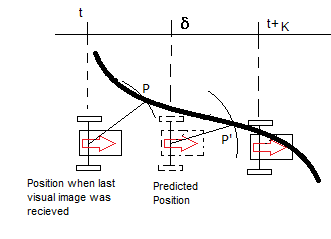
\includegraphics[width=.8\linewidth]{Chapter7/fig/robotPredictPos}
	\caption{Smith predictor applied to the developed mobile robot}
	\label{fig:SmithRobot}
\end{figure}
 \begin{figure}
	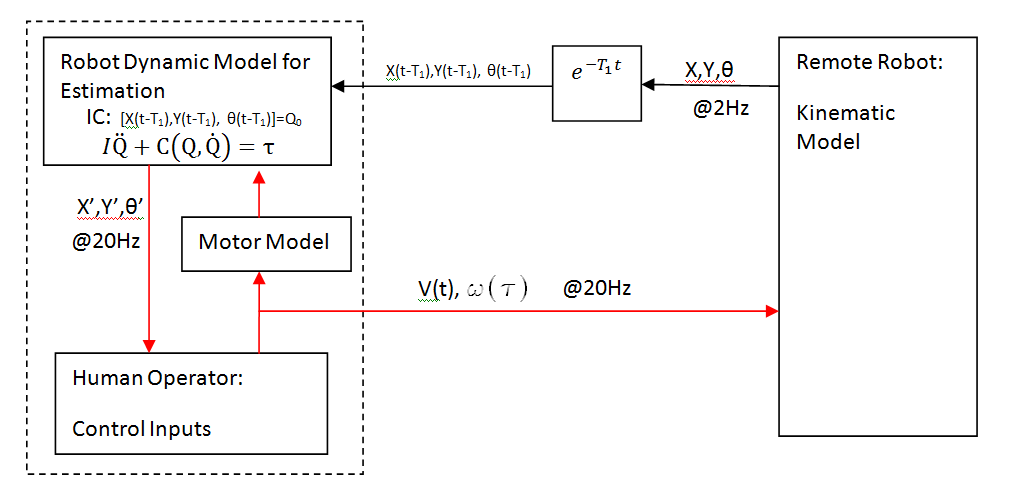
\includegraphics[width=\linewidth]{Chapter7/fig/Sumilation_BlkDgm}
	\caption{Simulation block Digram}
	\label{fig:SimBlock}
\end{figure}
\subsection{Simulation algorithm and  results} 
The simulation scheme is  shown in block digram of Figure \ref{fig:SimBlock}. The algorithm  is explained  below.

\begin{algorithmic}[1]
	\State Convert the path from global coordinate system (CS) to Robot's Local Coordinate System based on the  current pose  $(x,y,\theta)$ of the robot.
	\State With a given look ahead distance ($l$) search for a goal point on the path.
	\State Determine the turning radius ($r$) using Equation 6.5 
	\State Calculate $\omega$ using turning radius ($r$) and given Linear Velocity $v$
	\State Command Robot $\omega$ and  $v$
	\If  {new pose of the robot is available from remote station}
		\State Update robot pose $(x,y,\theta)$
	\Else
		\State Calculate the predicted pose of the robot  based on command given in Step 4, and using dynamic model of therobot given by Equation \ref{CE2}.
		\State Update robot's pose $(x,y,\theta)$ 
	\EndIf
	\State\textbf{ Goto} Step 1
\end{algorithmic}	
 Simulation was carried using Matlab. Differential equation solver \textit{"Ode24"} was used to solve Equations \ref{eqn:KinematicModelOfRobot} and \ref{CE2}.  The desired path  was a circle of radius 5m centred at origin of the global coordinate system. The human action was modelled with look ahead distance $l$ of 0.5m and linear velocity $v$ of $0.5~m/s$. The initial position of the robot was (4.5,0.0). 
 The  robot's motion  under feedback delay of 0.5 sec and 0.8 sec, i.e.,  $T_1=0.5~sec$ and $T_1=0.8~sec$,  are shown in  Figures \ref{fig:PreDelay500plot} and \ref{fig:PreDelay800plot} respectively.   It is seen that oscillation are no more visible at delay of 0.5 sec  and   0.8 sec. The system shows no instability. 

 \begin{figure}[h]
 	 \begin{minipage}[T]{0.5\linewidth}
 	 	\centering
 	 	\captionsetup{justification=centering}
 		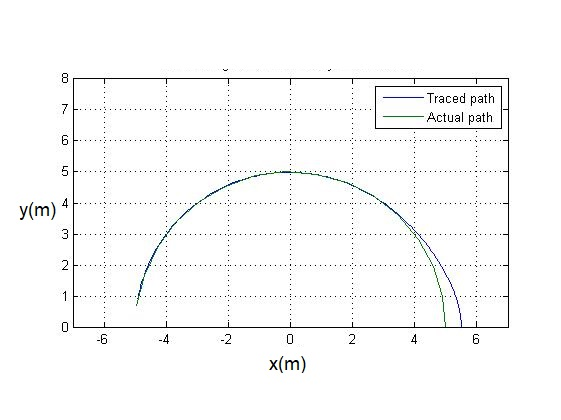
\includegraphics[width=\linewidth,keepaspectratio]{Chapter7/fig/withPrediction05dely}
 		\captionof{figure}{Time delay $T_1=.5~sec$\\ and $T_2=0$ }
 		\label{fig:PreDelay500plot}
 	\end{minipage}
 \hfill
 	\begin{minipage}[T]{0.5\linewidth}
 		\centering
 		\captionsetup{justification=centering}
		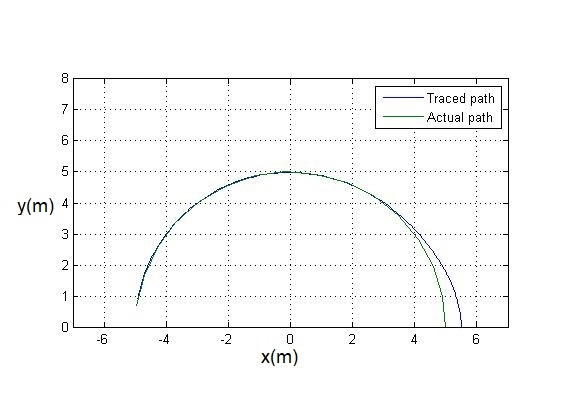
\includegraphics[width=\linewidth,keepaspectratio]{Chapter7/fig/withPrediction08delay}
		\captionof{figure}{Time delay  $T_1=.8~sec$ \\ and $T_2=0$ }
		\label{fig:PreDelay800plot} 
 	\end{minipage}
 \end{figure} 


The above results show that model-based prediction of the robot's pose helps in removing the instability of the system. In  actual teleoperation, the operator's control actions are based on the visual display available to him.  The delay in visual feedback results in inefficient operator's performance as the person tends to adopt a wait and watch policy to see the effect of his control action. In the next section,  an implementation and adaptation  of above discussed \textit{model based prediction }  for  visual display feedback is presented.   
  
\section{Delay Compensation using Predictive Display}
As indicated in  Literature survey,  the delay of visual feedback leads to inefficient and unstable performance of a teleoperated system. There are two major methods to overcome time delay induced problems in teleoperation. One is to use \textit{supervisory control} and the other is \textit{predictive display}. The second methodology, i.e., the Predictive Display, was adapted here. This is because it is more intuitive to human operators, and the onboard controller  required on the mobile robot is very much simplified.  

  
Predictive display has been defined as using the computer for extrapolating the display forward in time \cite{sheridan}. In this, a local model of the remote scene is used to predict and render the remote scene in response to operator's command. It replaces the delayed video feedback with extrapolated synthesised  image of the remote environment. This enables the operator to perform the task normally. Predictive display has been implemented in the past using different sensors such as monocular camera fixed on the wall, camera mounted on the robot arm, fusion of Lidar scanner and RGB camera, etc. 
The proposed approach here is to use a low-cost  Kinect Sensor from Microsoft Inc. to generate the 3-D model of the remote environment and use kinematic model of the mobile robot to predict the motion of the actual robot on the 3-D model of the environment  to generate a delay-free estimated image of the remote scene operator.

\subsection{The Kinect sensor }
\begin{figure}
	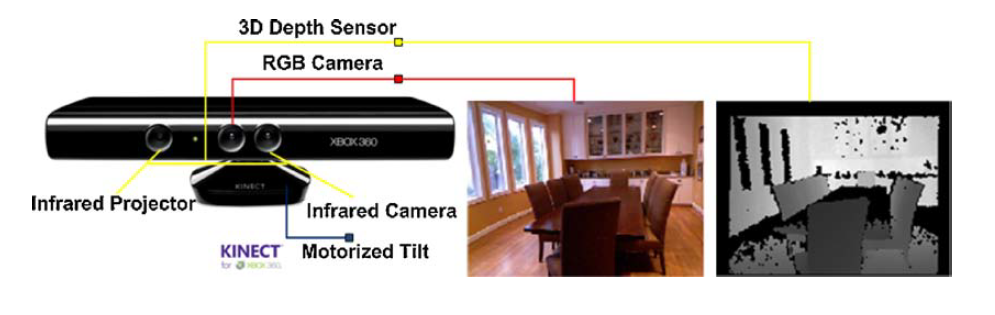
\includegraphics[width=\linewidth,keepaspectratio]{Chapter7/fig/Kinect}
	\caption{Kinect Sensor from Microsoft}	\label{fig:Kinect}
\end{figure}
Kinect sensor from microsoft is shown in Figure \ref{fig:Kinect}. The hardware contains a normal RGB camera, a depth sensor and a four-microphone array, which are able to provide  RGB images,  depth signals, and audio signals simultaneously. The depth sensor comprises of an Infra Red (IR) projector and the IR camera. The IR projector casts an IR speckle dot of known  pattern into the 3-D scene while the IR camera captures the reflected IR speckles. To determine the depth, triangulation method is used.  Kinect is therefore an instance of a structured light depth sensor. More details concerning the structured light 3-D imaging technology can be found in \cite{geng2011structured}. 

The \textit{RGB camera}  delivers three basic colour components of the video. The camera operates at 30 Hz, and can offer images at $640\times480$ pixels with 8 bits per channel. The  \textit{3-D Depth Sensor} creates a depth map, which provides the distance information between the camera and an object. The sensor has a practical range limit of 0.8m-3.5m distance, and outputs video at a frame rate of 30 frames/sec with the resolution of 640 x 480 pixels. The angular field of view is $57^o$ horizontally and $43^o$ vertically.
Number of different open source software libraries are available  which includes OpenNI \cite{openni}, Microsoft Kinect SDK  \cite{mssdk} and OpenKinect \cite{freenect} to access data from the Kinect sensor. OpenNi was used in this research, as it is compatible with RTabMap, an Open Source Software used for reconstruction of the 3-D point cloud model of the  remote scene. 

\subsection{Onboard data processing and transmission}
In teleoperation. the Kinect sensor mounted on the mobile robot was connected with the onboard Raspberry Pi single board computer with limited processing power. The onboard controller uses OpenNi library to interface with the kinect hardware.  The Kinect sensor has two separate cameras. The transformation between the camera centres are known and provided by the manufacturer. It therefore generates two streams, the colour and depth data. It is possible to send the two raw data streams over the network  without any processing at the robot's side. This  puts less stress on the onboard computer but requires high communication bandwidth. The other option is to stream \textit{ registered depth} data over the network. This requires less bandwidth as each pixel has both the colour and depth value associated with it when it is transmitted. Depth Registration requires minimal computing power. Known transformation between the two cameras was used to align the depth pixel and the colour pixel so that they correspond to the same point of the 3-D scene. This is referred to as \textit{depth registration} or \textit{image registration} in the literature. The word "depth" in the   \textit{depth registration} indicates  that the final image data is with respect to  the depth camera's frame. The second method was adapted here. The robot transmits registered depth data, i.e., the RGB and the Depth (RGB-D) values associated with each pixel to the control station over network. 


\begin{figure}
	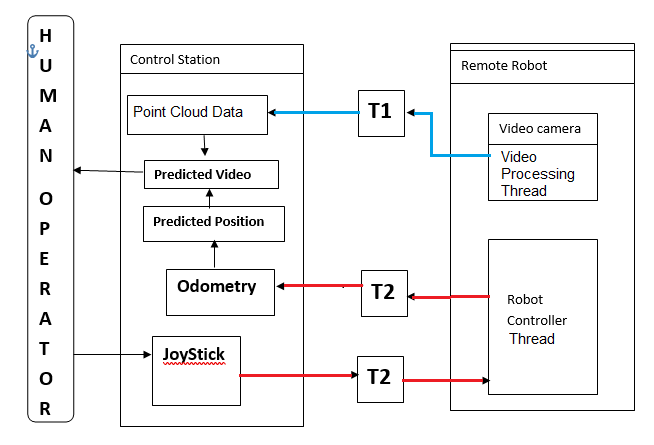
\includegraphics[width=\linewidth,keepaspectratio]{Chapter7/fig/PredictorBlockDig}
	\caption{Predictive display architecture}	\label{fig:PDBLock}
\end{figure}

\subsection{3-D reconstruction }
The registered depth data received at the operator-station was processed using the RTabMap library \cite{rtabmap} and 3-D Point Cloud data was generated. The details of the working of RTabMap can be found in \cite{labbertab} and \cite{labbe2013appearance}.  Point cloud map is a set of points in 3-D space derived using the camera model and the depth data associated with each pixel of the depth registered data sent from the mobile robot. Each new frame that arrives is added to the current data set after proper transformation. The transformation between the two frames of data was created by matching the common feature in the two frames. The RTabMap library thus outputs a set of 3-D point alongwith their RGB color. The coordinates of the points are always  with respect to camera coordinate frame. It may be noted that the registered depth image that has arrived was delayed by $T_1$ unit of time. So the local station always has a 3-D map w.r.t  the robot at $(t-T_1)$ sec.
 

\subsection{Extrapolation of remote scene } 
The visual data present in the current frame is the view that the robot has seen $T_1$ seconds earlier. Let this data be denoted as $P(t-T_1)=Set\{P_k\}$. The point $P_i$ is associated with the coordinates ${Px_k,Py_k,Pz_k}$ and color data $c_k$. In order to predict the current scene that the robot might be seeing one needs to estimate the current position of the robot. The dynamic model developed in chapter \ref{c4_Dynamics} is used to estimate the current position of the robot. To accomplish this the  architecture of the teleoperation shown in Figure \ref{fig:PDBLock} was developed and used to compensate for the time delay.
 It has been stated earlier that the delay $T_2$ in exchange of command data and the wheel velocity data from the robot to the operator station was 20ms. It may thus be assumed that  using the odometric data in Equation \ref{eqn:odo1},~\ref{eqn:odo2} and \ref{eqn:odo3}, the current position of the robot was always known to the operator-station. This was performed by Odometric Block of Figure \ref{fig:PDBLock} by using Equations \ref{eqn:odo1},~\ref{eqn:odo2} and \ref{eqn:odo3} from time $t-T_2$ to $t$. Where $t$ denotes the current time and  with initial condition \[x(i=0)=0,~y(i=0)=0 ,~ \beta(i=0)=0\] and  \[ i=0 \text{ to } n;  \quad n=T_1/T_2\] 
 Let the predicted position of the robot at time $t$ be given by 
\[[x(i),~y(i) ,~ \beta(i)]\rightarrow [_v(t),y_v(t),\beta_v(t)]^T\]
This was basically the amount by which the robot has moved after the last video frame had arrived. Next, the transformation matrix, $T^c_r$ between the mobile robot's coordinate frame at point $O_r$ in Figure \ref{fig:KenVec} and the camera frame was used to calculate the change in pose of the camera. Since the points $P_i$ are in the camera frame their current coordinates ${P'x_i,P'y_i,P'z_i}$ was arrived at by using 
\begin{eqnarray}
\begin{pmatrix}
P'x_i \\ P'y_i \\P'z_i
\end{pmatrix}=T^c_r
\begin{pmatrix}
Px_i\\Py_i\\Pz_i
\end{pmatrix}
\end{eqnarray}
This new location of the points were then  projected onto the screen of the local operator, thus, giving him the estimated current view of the remote scene. 
 \begin{figure}[ht]
	\begin{minipage}{.5\textwidth}
		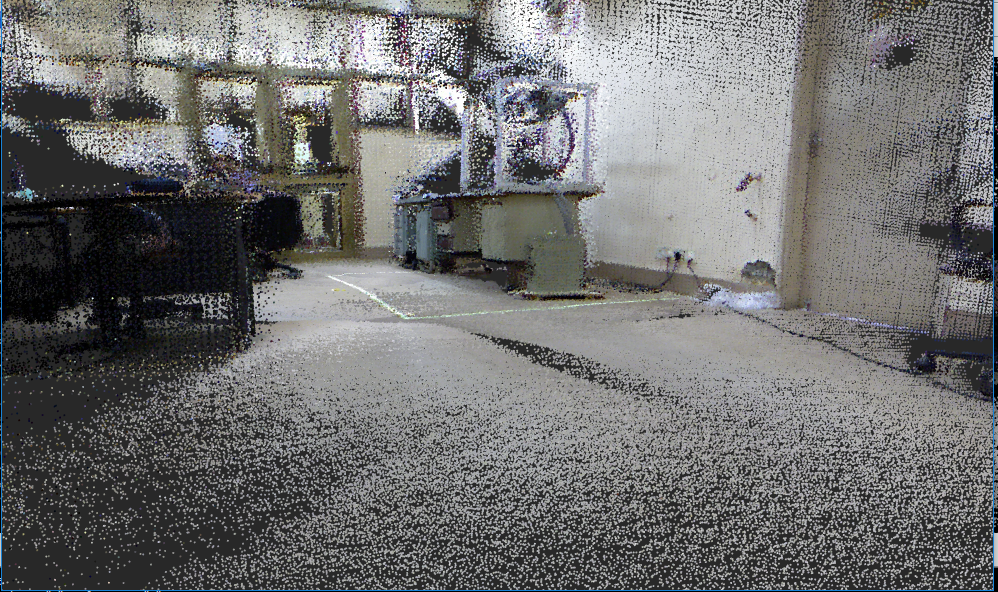
\includegraphics[height=4cm,keepaspectratio]{Chapter7/fig/pcdT}
		\captionof{figure}{PCD at time T }
		\label{fig:pcdt} 
	\end{minipage} 
	\begin{minipage}{.5\textwidth}
		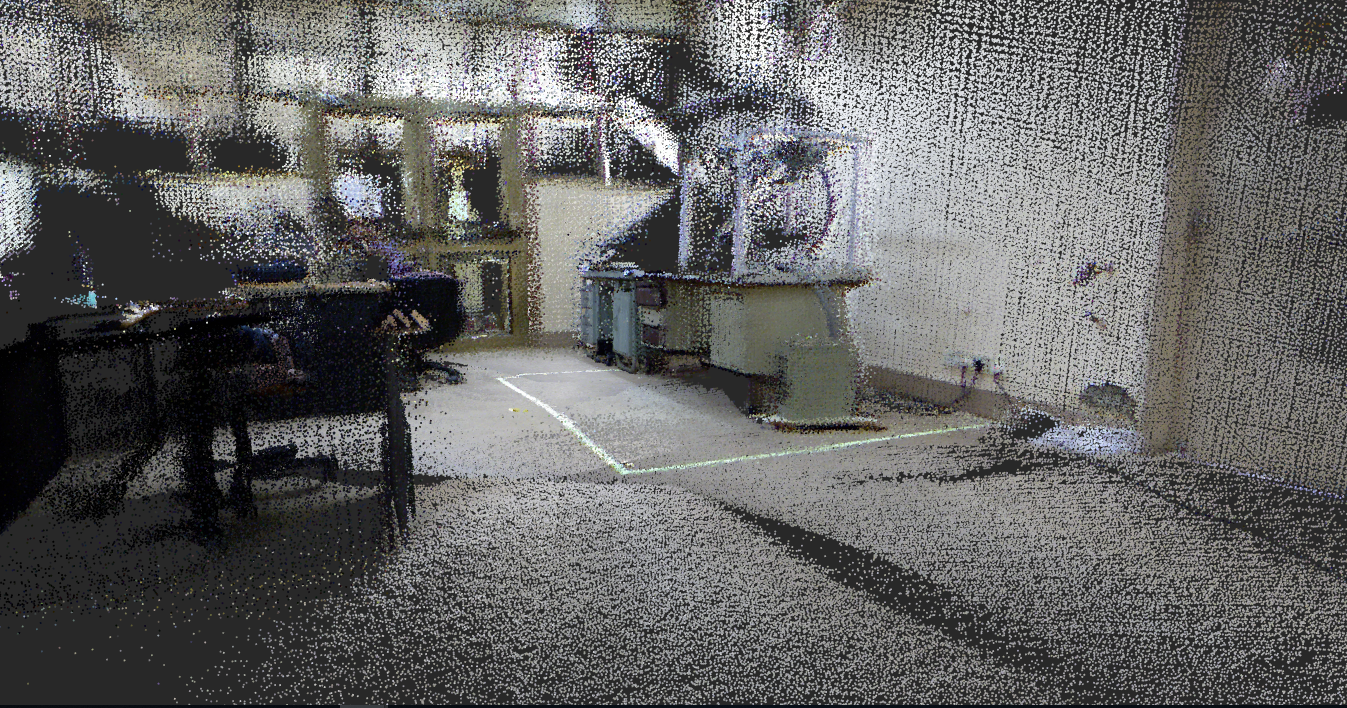
\includegraphics[height=4cm,,keepaspectratio]{Chapter7/fig/pcdT_p}
		\captionof{figure}{Predicted Scene}
		\label{fig:pcdP} 
	\end{minipage}
\end{figure}
The view available at the operator station at time $t$ is shown in Figure \ref{fig:pcdt} which is $T_1$ sec old. Based on this old data, the predicted scene is shown in Figure \ref{fig:pcdP}.  The operator  sees  Figure \ref{fig:pcdP} instead of Figure \ref{fig:pcdt}.

With the predictive display model the operator was able to move the robot without\textit{ "wait and see"} stratagey adopted earlier. The motions were smooth and speed of operation improved.

\section{Summary}
In this chapter,  the model-based predictive control for control of mobile robot over time delayed network is presented. The stability of the control was verified using simulation. This model was then adopted for  teleoperation using visual feedback. Kinect sensor was used to generate the 3-D model of the remote environment in real time. The estimated position of the mobile robot using the odometry was used to project a synthesised image of the 3-D model of the remote environment.  
